\documentclass[../main.tex]{subfiles}
\graphicspath{{\subfix{../src/}}}


\begin{document}
\section{Methodology \& Implementation}

\subsection{Anatomy}
\label{sec:anatomy}

The hand is an anatomically-complex appendage designed to facilitate a large amount of control in different usage scenarios.
The hand consists of 27 bones, 14 of these are called phalnages, and make up the 4 fingers and the thumb.
These bones, alongside a complex set of $\sim30$ muscles are able to perform $24$ Degree-of-Freedom (DoF) of rotational motion.
The individual finger consists of 3 bones called \gls{phalanges}, arranged linearly from the palm of the hand.
The 3 finger bones are called the proximal phalange, middle phalange and distal phalange.
The joints between the phalanges have 1 DoF and are able to do \gls{flexion/extension} movement, while the base of the finger have 2 DoF and are able to do \gls{flexion/extension} \& \gls{abduction/adduction} movement.
The anatomical muscle and joint structure of the hand/forearm can be seen in the figure \ref{fig:anatomy}.

\begin{figure}[h]
\begin{center}
\includegraphics[width=0.8\textwidth]{example-image-a}
\caption{A rendering of the anatomical muscle and joint strucutre of the lower-arm. The complexity of the muscles controlling the hand can be seen. Source \cite{???}}
\label{fig:anatomy}
\end{center}
\end{figure}

\subsection{Brief of used Software}
\label{sec:software}

In order to design a simulated prosthetic device that facilitates the requirements stated in section \ref{sec:prost_sim}, an effective simulation software needs to be chosen.
The software needs to be controllable from an external source, such as ROS, and because of this, software like Gazebo \cite{gazebo} or CoppeliaSim \cite{coppeliasim} is ideal.
Both simulation softwares allow for the creation of advanced dynamic-body simulations.
CoppeliaSim \cite{coppeliasim} was chosen due to its intuitive development workflow.

In order to record the joint movements of the hand, while simultaneously record the sEMG activity of the body, products that support hardware-synchonization needs to be used.
Products designed to capture sEMG data are widely spread.
As mentioned in the paper \cite{Zhaolong2021}, the Myo armband \cite{myo} or the Delsys Trigno package \cite{emgworks} could be used.
The Delsys Trigno \cite{emgworks} facilitates a hardware-synchonization recording mode out of the box, while the myo armband \cite{myo} does not.
Because of availability, and synchronization capabilities it is ideal to use the Delsys Trigno as the sEMG recording device.

Lastly, a product designed to capture the joint movements of the hand needs to be chosen.
A simple solution to hand tracking would be to use a software like MediaPipe \cite{mediapipe}, a python based landmark tracker that can track the joint angles of the hand using Machine Learning from a video feed.
An alternative is mentioned in the paper \cite{Zhaolong2021}, where a glove containing flex sensors could be used.
This approach would provide relieable joint angle data without relying on a camera setup.
Lastly, a capture glove could be fitted with 3D markers, detectable from a high-accuracy and high-framerate system such as the Motive motion capture setup \cite{optitrack} created by OptiTrack.
It was chosen to use the Motive setup due to availablility and the additional benefit of having a hardware-synchnonization feature, that can be combined with the Delsys Trigno \cite{emgworks} setup.


\subsection{Dataset Creation}
\label{sec:dataset}

In order to train a simulated hand prosthetic, a sofisticated dataset containing the measured relation between muscle activity and the finger placements is needed.
In order to create a dataset of the hand, it is important to choose a set of day-to-day movements the dataset should contain.
The paper \cite{KeunTaeKim2021} proposes the ``Southampton Hand Assessment Procedure'' (SHAP) \cite{shap} as its main method of dataset creation, an alternative would be the ``Sollerman Hand  Function Test''  \cite{sollerman}.
Both procedures are used in assessing the function and moveability of the human hand.
By analyzing the most important gripping motions in both tests, it should be possible to denote a suitable set of grips that the dataset needs to contain.
The sollerman grip types are ranked based on their usage percentage in activities of daily living.
From this, the most used grip types according to sollerman are the \textit{Pulp pinch}, \textit{Lateral pinch}, \textit{Five-Finger pinch} \& \textit{Diagonal Volar grip (Power grip)}, see \cite{sollerman} for further details.
SHAP also proposes a set of grip types that are used in day-to-day tasks, these are \textit{Spherical grip}, \textit{Tripod pinch}, \textit{Power grip} \& \textit{Lateral pinch}.
In order to create a dataset mimics the movements of day-to-day tasks, the most important grips from \cite{sollerman} \& \cite{shap} has been chosen.
The grip types that needs to be part of the dataset and their usage descriptions can be seen in table \ref{tab:grips}.
A set of consise grip types has been chosen as an alternative to a larger set of general grips.
This is done as a basis of creating a specialized dataset that would be easier to train and work with as a proof of concept.
%The chosen grips are chosen as a basis for the creation of a dataset. creating 

\begin{table}[h]
\begin{center}
\begin{tabular}{ |l|l| } 
 \hline
 Grip Type & Finger Usage Description \\ 
 \hline
 Pulp pinch & Between thumb, index and middle finger \\ 
 Lateral pinch & Between thumb \& side of index finger \\ 
 Five-Finger pinch & Between thumb, and all four fingers \\ 
 Power grip & Between thumb, and all four fingers with contact to palm \\ 
 \hline
\end{tabular}
\caption{The most used hand grips in day-to-day tasks based on \textit{Southampton Hand Assessment Procedure} \cite{shap} \& \textit{Sollerman Hand Function Test} \cite{sollerman}.}
\label{tab:grips}
\end{center}
\end{table}


\subsubsection{Existing datasets}

In addition to creating a dataset for this thesis, it would be intresting to compare with an existing state-of-the-art dataset.
The paper \cite{jarque2019} proposes the use of their dataset \cite{kinmusdataset}.
The dataset contains a very large set of recordings, consisting of precise anatomical angles of the hand, with the assosicated muscle activity of the forearm.
The dataset consists of $572$ recordings from $22$ subjects, in both reaching, gripping \& releasing actions.
Another dataset is explained in the paper \cite{ashirbad2022}, as an alternative of using finger joint angles as the ground truth data needed to train a network on sEMG data, the dataset uses a set of $16$ gesture classes for a classification algorithm.
The paper explains that the sEMG data in the dataset has been subject to a pre-processing step using a $10$ to $500Hz$ bandpass buttersworth filter, and in order to remove powerline noise a $60Hz$ notch filter was used.
The dataset was created on $43$ participants.

%The recording of the dataset is done using the software explained in section \ref{sec:software}, namely Motive \cite{motive} \& EMGworks \cite{emgworks}.
%TODO: Present more formally and mention company names.

\subsubsection{sEMG Sensor Locations on the Body}

To create a dataset that correlated muscle activity to the movements of the hand, it is important to choose a set of active muscles to record.
$\sim 30$ muscles are used in total to control the hand, but it would not be possible to record all of them simultaneously.
6 sEMG sensors were available in the Delsys Trigno \cite{trigno} system, and these needed to be placed optimally in order to increase recording of the most important muscles.
Target areas on the lower-arm for sEMG sensors are proposed by the paper \cite{jarque2019}.
Additionally, target areas of the upper-arm \& upper-body were chosen based on the suggestions from the paper \cite{Batzianoulis2018}.
The chosen muscles to record with sEMG sensors can be seen in table \ref{tab:muscletargets}.

\begin{table}[h]
\begin{center}
\begin{tabular}{ |l|l| } 
\hline
Muscle & Main Functionality \\ 
\hline
(A) \textit{Flexor Digitorum Superficialis} & Flex of the 4 fingers \\
(B) \textit{Extensor Digitorum} & Extension of the fingers \\
(C) \textit{Extensor Carpi Radialis Longus} & Wrist exstension \& hand abduction \\
(D) \textit{Triceps Brachii (long head)} & Extension of the arm \\
(E) \textit{Biceps Brachii} & Flexion of the arm \\
(F) \textit{Pectoralis Major / Frontal Deltoid} & Movement of the Arm \\
\hline
\end{tabular}
\caption{The muscles targeted with the 6 available sEMG sensors, as recommended by the papers  \cite{jarque2019} \& \cite{Batzianoulis2018}.
 The targeted muscles contributes to a lot of the movements of hand \& lower-arm, and are ideal for the dataset.
}
\label{tab:muscletargets}
\end{center}
\end{table}

The target muscles were chosen as they contribute to a lot of the overall movements of the hand \& lower-arm.
The muscles in table \ref{tab:muscletargets} are numbered, and the locations of the individual sensor with the corresponding muscle can be seen in figure \ref{fig:musclesensors}.

\begin{figure}[h]
\begin{center}
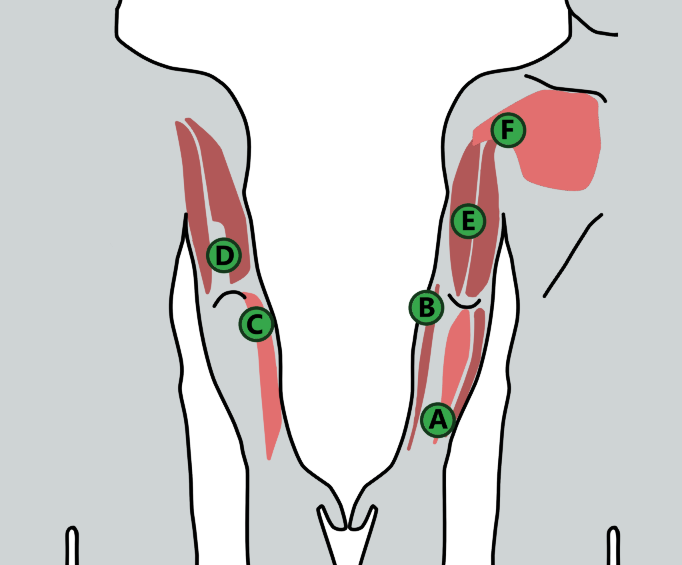
\includegraphics[width=0.8\textwidth]{muscletargets.png}
\caption{Muscle diagram, containing the target sEMG locations. The numbering corresponds to the muscle names in table \ref{tab:muscletargets}. The left image shows the muscles on the rear of the arm, while the right shows the muscles on the front of the arm.}
\label{fig:musclesensors}
\end{center}
\end{figure}
%TODO: Image is not final, might require adjustments..

It was chosen to split the amount of sensors evenly along the lower-arm and the rest of the body in order to asses how important the different muscles are in prediction of the hand.

\subsubsection{Motion Capture Glove}

The motive capture system created by OptiTrack is a set of 8 high-quality cameras mounted to cover a target capture area.
%TODO: how many cameras were there?
The capture system detects flouresent 3D markers in the given capture area, with the purpose of triangulating the markers and effectively calculate 3D poses for the markers in the scene down to an effective accuracy of $\pm 0.2mm$ \cite{motive}.
In order to get precise recordings of the motion of the hand and fingers, flourecent 3D markers were placed on a glove.
The pattern of the marker positions were closen in order to calculate the angles of the individual finger bones.
The markers are used in sets of 3, this allows for the calculation of the triangle angles in 3D space.
The positions of the 3D markers on the recorder glove can be seen in figure \ref{fig:glove}.
An example of flexion with the capture glove can be seen in figure \ref{fig:glove_flex}.


\begin{center}
\begin{figure}[h]
\includegraphics[width=0.8\textwidth]{example-image-a}
\caption{The positions of 3D markers on the capture glove, designed to be detectable using the  Motive Capture software \cite{motive}.}
\label{fig:glove}
\end{figure}
\end{center}

\begin{center}
\begin{figure}[h]
\includegraphics[width=0.8\textwidth]{example-image-a}
\caption{Flexion of the index finger and its transformation of the 3D markers on the capture glove.}
\label{fig:glove_flex}
\end{figure}
\end{center}

\subsubsection{Problems with Motive Tacking Software \& Capture Glove}
\label{sec:motiveproblems}

During testing and the creation of the dataset, several problems with the capture glove design and the capture setup became apparent.
These problem severely reduced the amount of time available to create and process a large dataset for this thesis.
The Motive Motion Capture software \cite{motive} had a lot of difficulty with finding, recording and optimizing the 3D markers placed on the capture glove.

The  Motive sofware used to generate the 3D poses is designed to detect 3D markers in the scene.
Once the markers are found in the individual cameras, they are subject to an optimization algorithm that effectively tries to determine if the markers seen in 1 camera is the same as the markers in the other cameras.
The first problem that occoured was specular reflection in the scene caused by shiny surfaces redirecting light in the target area.
This creates \textit{phantom} markers that can be seen in only a small set of frames.
Another problem with the capture setup is the optimization algorithm.
During recording of the dataset, it became apparent that it would not be possible to recort multiple fingers at the same time.
3D markers very close to each other seemed to be connecting, and only become a single marker in the tracking software.
This problem specifically occoured when the markers at the finger tips of the glove came in contact with each other causing marker data to be lost.
Furthermore, the Motive Capture software uses an auto-labeling system that is able to determine if the markers seen in one frame, are the same markers in the next frame.
This system proved to only be semi-relieable, giving labeled marker sequences of less than $\sim 200$.
During a sequence of 15 seconds of recording, a set of 7 markers in the scene became over $100$ labeled marker tracks. And the problem increased as 30 seconds of fotage could create up to 1000 marker labels.
The unreliable labeling of markers can be seen in appendix \ref{appendix:motivefixing}.

%TODO: Mention that markers needs to be very close (2-3 cm) and this might not be intended for motive software.


\subsubsection{Reduction of Tracking Software Problems}

%In order to fix some of the problems, caused by the setup, software was written.
%TODO: shitty starter
The large amount of problems observed using the Motive Motion Tracking software makes it impossible to use the tracking output as training data.
The problems requires the user to manually combine labeled marker sections into larger labeled sections, in order to reduce changing labels on the tracked markers.
It would be ideal if this functionality existed in the Motive software, but this was not the case.
Because of a lack of functionality in Motive, software was created to replay the 3D markers in real-time, with their associated labels.
Furthermore, software that was able to remove, merge and subsample markers was used to clean the labels.
The software created to fix unreliable labeling of markers can be seen in appendix \ref{appendix:motivefixing}.

%TODO: Muscles of the hand: https://www.assh.org/handcare/safety/muscles
%TODO: Bones of the hand: https://www.bidneedham.org/departments/orthopaedics/hand-program/anatomy-hand-and-wrist
\subsection{Design of a Simulated Prosthetic Hand}
\label{sec:prost_sim}

In order to design a state-of-the-art simulated prosthetic hand, a number of anatomical design choises needs to be considered.
This thesis tries to create the most anatomically-correct hand simulation available, this will hopefully have a number of positive effects on prosthetics research.
By having access to an advanced simulation, it would in turn be able to test and visualize more advanced movement controllers that can facilitate more DoF than current commercial prosthetics. 
By creating an anatomically correct prosthetic hand simulation, it is hoped that prosthetics users can have more advanced rehabilitation, and learn to have more natual control of their prosthetics. This would create a more natual usage experience, and decrease the percentage of users that reject the usage of their prosthetic alltogether.
A set of requirements The simulated anatomically correct hand should be determined in order to create a state-of-the-art prosthetics simulation.
The simulated prosthetic should:

\begin{enumerate}
\item Facilitate the same DoF as an anatomically correct hand.
\item Have porpotions that closely resemble that of an anatomically correct hand.
\item Be simulated and be controllable in a commonly used robotics software to increase accesability for researchers.
\end{enumerate}

The resulting prosthetic hand simulation can be seen in appendix \ref{appendix:handsim}.

\subsubsection{Simulated Hand Articulation design}

%TODO: see Yuki2023 (page 11) for how to properly show the dimensions of my hand!
In order to translate the biology and anatomy of a real hand explained in \ref{sec:anatomy} into an robotics simulation, we start by denoting the relative lengths of the wrist bones and phalnages by refrence, as can be seen in figure \ref{fig:handref}.

%TODO: IMAGE HERE OF HAND OR XRAY
\begin{figure}[h]
\begin{center}
\includegraphics[width=0.8\textwidth]{example-image-a}
\caption{Example figure text}
\label{fig:handref}
\end{center}
\end{figure}

The porpotions of the refrence is used to denote the bone lengths for the model.
The model is implemented in Coppeliasim \ref{???}, The model is created in a hierachy, the bones are created with cylinders and the joints are created using 1 DoF Revolute joints.
% Ref coppeliasim
As specified in section \ref{sec:anatomy}, some joints of the human hand facilitates 2 DoF of rotation.
This is needed in order for the wrist and finger base joints to be able to do \gls{abduction/adduction}.
To simulate this, two 1 DoF revolute joints were placed in series, thus allowing 2 DoF.


% \section{Implementation}

Based on the literature review in Section \label{sec:literature}, it becomes apparent that there exists a standard pipeline for translating sEMG recordings into predicted motorcontrol for a prosthetic.

\subsection{sEMG Data Processing}

Raw sEMG data contains a lot of unwanted noise as explained in section \ref{sec:noise}.
Some of the noise can be can be removed through signal processing using filters.
State-of-the-Art papers use a lot of different methods to reduce noise in sEMG data.
The paper \cite{multdof} proposes the use of a $50Hz$ Notch filter, while papers \cite{graspintent} \& \cite{ashirbad2022} respectively chooses a $20Hz$ cutoff Buttersworth filter \& a $10-500Hz$ band-pass Buttersworth filter, lastly the paper proposes a $60Hz$ notch filter in order to remove powerline noise.
Due to me many different filtering types used in state-of-the-art, it was determined that the use of a filter depends on the specific sEMG data, and that the best filter for this thesis is to be determined through testing.

%TODO: Convert n sEMG angles into a image heat map kinda, and compare before and after different filters? the z dimension could be change in values?

\subsection{Network Design}

\subsubsection{Window-Based Neural Network Designs}

%TODO: needs sources for this stuff?

%TODO: Some introduction and explanation of MLP and CNN types of networks.
%TODO: Go back and see what papers uses CNN's
Neural Networks are widely used in the field of AI.
One type of widely used neural network is a fully-connected Multi-Layer Perceptron (MLP) Network.
The MLP network is popular due to its structure and training capabilities.
A MLP consists of layers of weighted activation functions where each activation function in a layer recieves the entire previous layer's output summed up as input.
Due to the structure of a MLP, the network is capable of recieving a set of inputs and be trained to approximate a n'th degree polynomial function that relates the given inputs and outputs.
The network is trained by updating the individual weights through backpropagation with the predicted output and a ground-truth output.
The MLP network could be used to predict the relation between muscle activity and finger movements.

An alternative to a MLP that is similar in functionality is a Convoluted Neural Network (CNN).
A CNN consists of a set of Convolutional Layers that deforms inputs to abstract convolution features.
The structure is considered sparcely connected due to the convolution layers are only recieving a subset of the previous convolution features.
The feature conversion is ideal when a network needs to become robust and needs to recognize larger concepts in the input.
This functionality is especially used when the input data takes the shape of a matrix.
Once the input is convoluted to a chosen feature abstraction, it is given to a MLP strucure trained to convert the convolution features into a useable output.

MLP \& CNN networks have no time-based functionality, they recieve a set of inputs and produce an output.
Because of this, the sEMG muscle activity is segmented into windows of a decired size, the output angles are then chosen to be the first angle after the window.
Furthermore, due to the training dataset \cite{kinmusdataset} from section \ref{sec:dataset},  containing joint angles as ground truth, both methods are trained as regression networks rather than classification networks, and are trained using Mean Square Error (MSE) loss.

%TODO: Images of these for better clarity!!!!

\subsubsection{Recurrent Neural Network Designs}

Network types ideal for time-based data are Recurrent Neural Networks (RNN).
RNN networks are similar to MLP's with the main difference being that a RNN keeps a hidden memory state that is derived from earlier inputs.
This functionality makes RNN networks ideal for concurrent, time-based systems where a sequencial input distribution needs to be converted to a output regression.  
Additionally, since the RNN network does not use a window of data, it would be able to have a quicker response time than a MLP or a CNN.

A variant of a RNN can contain a special kind of hidden memory called Long Short Term Memory (LSTM).
a LSTM uses gates as a way of containing a memory.

%TODO: Some introduction and explanation of RNN and LSTM types of networks.
%TODO: Go back and see what papers uses these.

\subsubsection{Machine-Learning Designs}

%TODO: Some introduction and explanation of feature extraction, what types and papers that uses these.
%TODO: Some introduction and explanation of SVM and LDA types of networks.
%TODO: Go back and see what papers uses these.

%\subsection{Software Hand Design}

\end{document}
